%%%% ijcai19.tex

\typeout{IJCAI-19 Instructions for Authors}

% These are the instructions for authors for IJCAI-19.

\documentclass{article}
\pdfpagewidth=8.5in
\pdfpageheight=11in
% The file ijcai19.sty is NOT the same than previous years'
\usepackage{ijcai19}

% Use the postscript times font!
\usepackage{times}
\usepackage{soul}
\usepackage{url}
\usepackage[hidelinks]{hyperref}
\usepackage[utf8]{inputenc}
\usepackage[small]{caption}
\usepackage{subfig}
\usepackage{graphicx}
\usepackage{amsmath}
\usepackage{booktabs}
\usepackage{algorithm}
\usepackage{algorithmic}
% \usepackage{epstopdf}
\usepackage{makecell}
\usepackage{float}
\urlstyle{same}

\usepackage{tikz}
\usetikzlibrary{calc}

% the following package is optional:
%\usepackage{latexsym}

% Following comment is from ijcai97-submit.tex:
% The preparation of these files was supported by Schlumberger Palo Alto
% Research, AT\&T Bell Laboratories, and Morgan Kaufmann Publishers.
% Shirley Jowell, of Morgan Kaufmann Publishers, and Peter F.
% Patel-Schneider, of AT\&T Bell Laboratories collaborated on their
% preparation.

% These instructions can be modified and used in other conferences as long
% as credit to the authors and supporting agencies is retained, this notice
% is not changed, and further modification or reuse is not restricted.
% Neither Shirley Jowell nor Peter F. Patel-Schneider can be listed as
% contacts for providing assistance without their prior permission.

% To use for other conferences, change references to files and the
% conference appropriate and use other authors, contacts, publishers, and
% organizations.
% Also change the deadline and address for returning papers and the length and
% page charge instructions.
% Put where the files are available in the appropriate places.

\title{Watercolor rendering and caustics effect for underwater scene} % TODO: TRANSLATE TO FRENCH MAYBE

% Multiple author syntax (remove the single-author syntax above and the \iffalse ... \fi here)
% Check the ijcai19-multiauthor.tex file for detailed instructions

\author{
Arnaud Paré-Vogt
\and
Mehdi Chaid
\affiliations
Département GIGL Polytechnique Montreal\\
\emails
arnaud.parevogt@gmail.com, % TODO: UPDATE WITH POLYMTL EMAIL
mehdi.chaid@polymtl.ca
}

\begin{document}
\makeatletter
\g@addto@macro\@maketitle{
  \begin{figure}[H]
  \setlength{\linewidth}{\textwidth}
  \setlength{\hsize}{\textwidth}
  \centering
  \centering
  \subfloat[Scene with simple diffuse light.]{
      \includegraphics[width=0.32\linewidth]{imgs/base_scene.jpg}\label{fig:base_scene}
  }
  \hfill
  \subfloat[Scene with watercolor effects.]{
      \includegraphics[width=0.32\linewidth]{imgs/watercolor_scene.jpg}\label{fig:watercolor_scene}
  }
  \hfill
  \subfloat[Final scene with all effects.]{
      \includegraphics[width=0.32\linewidth]{imgs/all_scene.jpg}\label{fig:all_scene}
  }
  \caption{Final underwater scene with multiple levels of effects.}
  \label{fig:project_results}
  \end{figure}
}
\makeatother
\maketitle

\begin{abstract}
Watercolor rendering is a unique non-photorealistic rendering (NRP) technique, 
used to simulate hand painting art on a 3D scene. In this paper, we attempt to
combine the effects of watercolor rendering with additional caustics and underwater
effects in order to produce an abstract scene with a swimming fish in OpenGL. 
Figure \ref{fig:project_results} shows the resulting scene with various levels of effects applied.

\end{abstract}

\section{Introduction}

The use of watercolor in the 3D industry is rare and usually limited to static images. 
It  goes again the general trend to make environments more realistic and detailed. This unique style, 
on the other hand, allows for some interesting variations of saturation and brightness, as well as vibrant, 
eye-catching colors that no other medium can match. Creating pleasant watercolor results requires 
careful planning, as well as a great deal of artistic understanding and experience. \medskip \par

\noindent
When used properly, this mix of bright, dancing colors and textured brush strokes creates images that appear 
simple at first glance, while retaining a surprising amount of details. As such, this style is often used in
architectural visualisation to produce rich images that allow for a quick understanding of the content, as can 
be seen in Figure \ref{fig:watercolor_architecture}.

\begin{figure}[h]
    \centering
    \subfloat[Dark, narrow street in \centering London.]{\includegraphics[width=0.4\columnwidth]{imgs/watercolor_architecture.jpg}\label{fig:f1}}
    \hfill
    \subfloat[Ponte San Angelo \centering ©Gerald Fritzler.]{\includegraphics[width=0.4\columnwidth]{imgs/watercolor_architecture_2.jpg}\label{fig:f2}}
    \caption{Watercolor style for architectural visualisation}
    \label{fig:watercolor_architecture}
\end{figure}

\noindent
Please note, however, that these examples were produced in a watercolor style that differs from the one 
presented in this paper.

\medskip \par
\noindent
Our main inspiration for this work comes from our wish to experiment with cel shading in an underwater 
scenery. While looking for reference material, we stumbled upon a relevant video that implement
this effect using Blender \cite{caustics_video}. We decided to push the idea further by mixing in a watercolor
effect as additional passes on top using a paper from \cite{watercolor_paper}.

\begin{figure}[h]
    \centering
    \subfloat[]{\includegraphics[width=0.45\columnwidth]{imgs/wp_result_1.jpg}\label{fig:wp1}}
    \hfill
    \subfloat[]{\includegraphics[width=0.45\columnwidth]{imgs/wp_result_2.jpg}\label{fig:wp2}}
    \caption{Some results from the reference watercolor paper.}
    \label{fig:watercolor_architecture}
\end{figure}

\medskip \par
\noindent
In this paper, we present a brief overview of the scene content, and project framework. 
We then go over the general pipeline used to produce the results in Figure \ref{fig:project_results}, before
diving into the implementation details of each step in their specific section. Lastly, some interesting 
results and research discussion will be mentionned, before concluding.

\section{Scene}

\subsection{Framework}

The source code for the project can be found on Github \cite{watercolor_underwater}. 
The code was written in C++ with OpenGL 4.6 core. We've used the LearnOpenGL \cite{learnopengl} 
online resource to bootstrap some of the initial work (camera class, shader class, model loading).

\subsection{Content}
The scene models an underwater environment with multiple static low polygon meshes scattered around. 
The floor is made of a square displaced patch produced in Blender, with a sand texture on top. 
All objects used in this project were not modeled by us, and are available for free on CgTrader \cite{cgtrader}.

\medskip \par
\noindent
In addition, an animated low polygon fish is placed in the water above. 
Only the sand plane model is textured, all other models use a constant color per face. 
Figure \ref{fig:scene_content} shows the models of the underwater scene without any effect applied on them.

\begin{figure}[h]
    \centering
    \includegraphics[width=.9\columnwidth]{imgs/scene_contents.png}
    \caption{Content of the scene with diffuse light.}
    \label{fig:scene_content}
\end{figure}

\subsection{Pipeline}

In order to draw an underwater scene, multiple effects must be combined together. This section provides an overview of the rendering pipeline of the project, and explains how each effect has been integrated in the pipeline. For more information about a specific effect, refer to one of the sections below.

Three main effects are added to the scene, and in addition, a very simple shadow map adds some realism. The main effects are enumerated below.
\begin{enumerate}
	\item Caustics
	\item Shadow map
	\item Watercolor rendering
	\item Underwater effects
\end{enumerate}

The ordering of all render passes is shown in figure~\ref{fig:render_passes}. Note that a render pass is defined by a series of draw calls that render to a given target. In our case, all render passes except the last one render to framebuffers. The correspondence between render passes and the corresponding effects is described below.


\begin{figure}[h]
	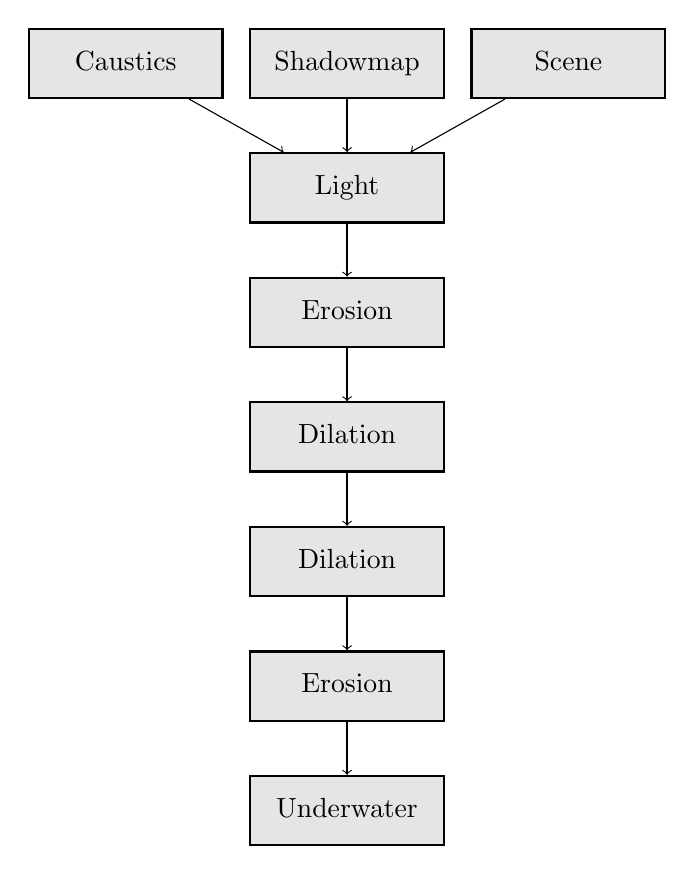
\begin{tikzpicture}[
	renderpass/.style={rectangle, draw=black, fill=black!10, thick, minimum height=2.5em, minimum width=7em, text height=height{"A"},text depth=depth{"g"}},
	]
	\node[renderpass] at (0, 0) (caustics) {Caustics};
	\node[renderpass] at (8em, 0) (shadowmap) {Shadowmap};
	\node[renderpass] at (16em, 0) (scene) {Scene};
	
	\node[renderpass] at (8em, -1 * 4.5em) (light) {Light};
	\node[renderpass] at (8em, -2 * 4.5em) (erode) {Erosion};
	\node[renderpass] at (8em, -3 * 4.5em) (dilate) {Dilation};
	\node[renderpass] at (8em, -4 * 4.5em) (dilate2) {Dilation};
	\node[renderpass] at (8em, -5 * 4.5em) (erode2) {Erosion};
	\node[renderpass] at (8em, -6 * 4.5em) (underwater) {Underwater};
	
	\draw[->] (caustics) to (light);
	\draw[->] (shadowmap) to (light);
	\draw[->] (scene) to (light);
	\draw[->] (light) to (erode);
	\draw[->] (erode) to (dilate);
	\draw[->] (dilate) to (dilate2);
	\draw[->] (dilate2) to (erode2);
	\draw[->] (erode2) to (underwater);
	\end{tikzpicture}
	\caption{schema of all the render passes in the program}
	\label{fig:render_passes}
\end{figure}

The caustic effect (further described in section~\ref{sec:caustics}) works as follows: it renders a caustic texture on a framebuffer and then projects the texture on the scene. This effect therefore requires a separate pass and a dedicated framebuffer for the texture to be rendered in.

The shadowmap works in much the same way, it renders a depth buffer in the point of view of the light, and then a check is made when drawing the light (note that the caustics are part of the light) to see if a given fragment is illuminated or not. Our shadow map implementation is very simple, and does not do a lot of work to obtain good-looking shadows. In practice, the watercolor effect is very prominent, so the irregularities are not very visible.

The caustic texture and the shadow map are applied on the scene in a separate pass, the "Light" pass. We use deferred rendering to calculate the illumination of the scene, so the light pass requires the position, normals and base colors for every fragment of the scene. The "Scene" pass is responsible for drawing all objects of the scene in order to retrieve the position, normal and color information per pixel and send it to the light pass.

The watercolor effect (further described in section~\ref{sec:watercolor}) is a bit more complicated. In order to be able to correctly apply the effect, we need to be able to sample neighbouring pixels. In order to do this, the effect is split in multiple passes. Stating from the light pass, 4 passes perform erosion and dilation effects. Then, the rest of the watercolor effect is applied at the same time as the underwater effects, in the underwater pass.

Finally, the underwater effect (further described in section~\ref{sec:underwater}) is applied at the end of the pipeline, in the underwater pass. The underwater effect is therfore computed in the same shader as the end of the watercolor effect. The result is rendered directly on the screen and completes the render pipeline.


\newpage
\section{Watercolor rendering}
\label{sec:watercolor}

TODO: Talk about the watercolor rendering pipeline here.

\subsection{Cel shading}

TODO: Talk about cel shading here.

\subsection{Normal smoothing}

TODO: Talk about normal smoothing here.

\subsection{Morphological smoothing}

TODO: Talk about morphological smoothing here.

\subsection{Paper effects}

TODO: Talk about paper effects here.

\subsection{Edge darkening}

TODO: Talk about edge darkening here.

\subsection{Pigment density variation}

TODO: Talk about pigment density variation here.

\newpage
\section{Caustics}
\label{sec:caustics}

In order to render caustics, we use a method called Periodic Caustic Textures \cite{periodic_caustic_textures}. This method is relatively simple. First, a grid with a certain resolution is generated. The grid is then rendered on a framebuffer. The vertex shader used in the rendering changes the x and y coordinates of the grid vertex by refracting the vertex as if it was a ray of light coming from above. The distorted mesh is then drawn in the fragment shader, using the ratio of the new area of a triangle over the original area of a triangle to calculate the color. This way, if the vertices are sent close together, the caustic color approaches white, while if the vertices are sent apart, the caustic color approaches black.

Figure \ref{fig:caustics_texture} shows the caustic texture generated by this approach.

\begin{figure}[h]
 \includegraphics[width=\columnwidth]{imgs/caustics_texture.png}
 \caption{caustic texture generated from our implementation}
 \label{fig:caustics_texture}
\end{figure}

In order to generate this texture, we must be able to refract and project on the ground the grid vertices. This means that we need access to a water height and a water normal. We do this by generating fractal noise (in our case 3 layers of Perlin noise) to get the water height, and then we use the finite element difference method to compute the normal. All this work is done in the vertex shader. In order to generate the Perlin noise, an implementation from Stefan Gustavson was used \cite{perlin_noise}.

Once the caustic texture is generated, we project the texture on the scene to give the impression that the scene is illuminated by the caustics. This is an approximation, but the result is good enough. Figure \ref{fig:scene_with_caustics} shows the scene with the caustics projected on it.

\begin{figure}[h]
 \includegraphics[width=\columnwidth]{imgs/scene_with_caustics.png}
 \caption{scene with the projected caustic texture}
 \label{fig:scene_with_caustics}
\end{figure}

\section{Underwater effects}
\label{sec:underwater}

TODO: Talk about underwater effects here.

\section{Results}

TODO: Showcase more results here.

% \newpage
\section{Future Work}

TODO: Talk about possible improvements here.

\section{Conclusion}

TODO: Conclude here.

\newpage
\appendix

%% The file named.bst is a bibliography style file for BibTeX 0.99c
\bibliographystyle{named}
\bibliography{ijcai19}

% The reference section will autofill when we add \cite{} in the report.

\end{document}

